
\begin{multicols*}{2}



\section{Barbarian}

\lettrine[lines=3, lhang=0.15, loversize=0.25, findent=.5em]{B}{arbarians} are tired of the empty battles they once craved. They wander, outcast, while their tribes curse the gods who abandoned them. They are consumed with rage and longing for foes worthy of their rage.

\subsection*{Rage}

In battle, you fight with primal ferocity. On your turn, you can use one point of stamina to enter a rage as a bonus action.



While raging, you gain the following stats if you aren’t wearing heavy armor:


\begin{itemize}
    \item You have advantage on Strength checks and Strength saving throws.
    \item When you make a melee weapon attack using Strength, you gain +2 bonus to the damage roll. The bonus increases to +3 at level 6th.
    \item You have resistance to bludgeoning, piercing, and slashing damage.
    \item If you are able to cast spells, you can’t cast them or concentrate on them while raging.
\end{itemize}


Your rage lasts for 5 turns. It ends early if you are knocked unconscious. You can also end your rage on your turn as a bonus action.



\subsection*{The Beast Within}

\subsection*{Feral Instinct}

By 7th level, your instincts are so honed that you have advantage on initiative rolls.

Additionally, if you are surprised at the beginning of combat and aren’t incapacitated, you can act normally on your first turn, but only if you enter your rage before doing anything else on that turn.

\subsection*{Relentless}

Starting at 9th level, your rage can keep you fighting despite grievous wounds. If you drop to 0 hit points while you’re raging and don’t die outright, you can make a DC 10 Constitution saving throw. If you succeed, you drop to 1 hit point instead.

Each time you use this feature after the first, the DC increases by 5. When you finish a short or long rest, the DC resets to 10.


\begin{Figure}
\centering
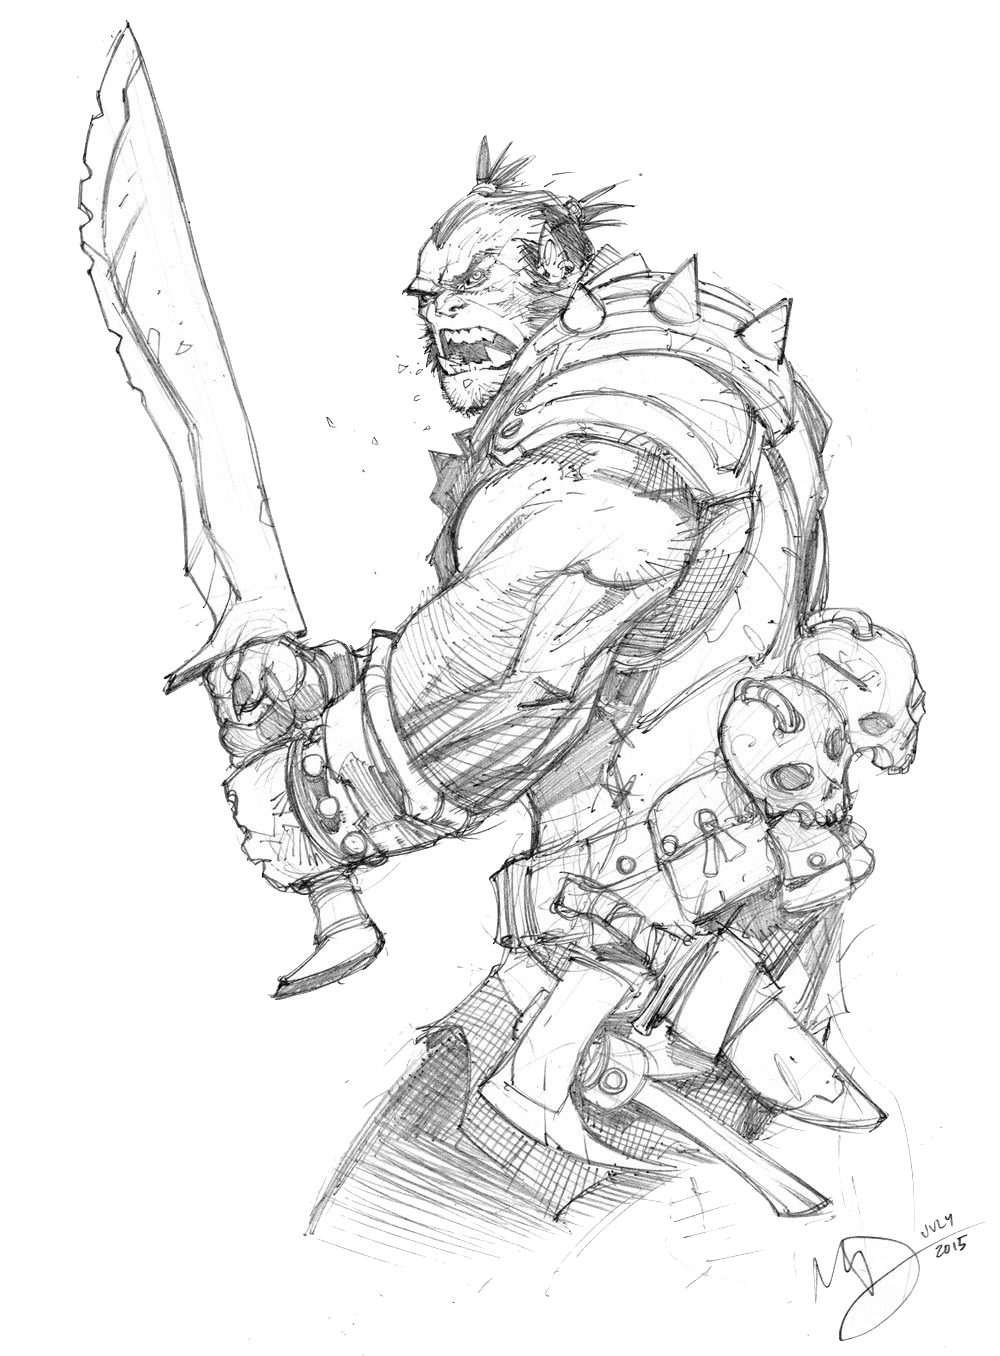
\includegraphics[width=\textwidth]{img/barbarian-half-orc.png}
\end{Figure}
    
\end{multicols*}